\documentclass[12pt, a4paper]{article}

% ==========================================
% 1. KHAI BÁO GÓI THƯ VIỆN (PACKAGES)
% ==========================================
% Bảng mã & Font chữ
\usepackage[utf8]{inputenc}
\usepackage[T5]{fontenc}

% Toán học
\usepackage{amsmath, amssymb}

% Căn lề & Bố cục trang
\usepackage[top=2.2cm, bottom=1.5cm, left=1cm, right=1cm, headheight=15pt]{geometry}
\usepackage{fancyhdr}
\usepackage{needspace}
\usepackage{tkz-tab}

% Đồ họa & Màu sắc
\usepackage{xcolor}
\usepackage{graphicx} 
\usepackage{tikz}
\usetikzlibrary{calc, shapes.geometric, positioning}


% Bảng biểu & Danh sách
\usepackage{colortbl}
\usepackage{array}
\usepackage{makecell}
\usepackage{multirow}
\usepackage{tasks}

% Biểu tượng
\usepackage{fontawesome5}

% ==========================================
% 2. THIẾT LẬP MÀU SẮC CHỦ ĐẠO
% ==========================================
\definecolor{goldyellow}{RGB}{255, 179, 0}
\definecolor{amberorange}{RGB}{230, 115, 0}
\definecolor{lightamber}{RGB}{255, 248, 225}
\definecolor{deepblue}{RGB}{25, 42, 86}
\definecolor{accentred}{RGB}{232, 65, 24}
\definecolor{softgray}{RGB}{220, 220, 222} 
\definecolor{fbblue}{RGB}{15, 80, 200}


% ==========================================
% 3. CẤU HÌNH HEADER & FOOTER
% ==========================================
\pagestyle{fancy}
\fancyhf{}
\renewcommand{\headrulewidth}{0pt}

% Khai báo biến lưu trữ nội dung góc phải của Header
\newcommand{\HeaderRightText}{}

% --- Header ---
\fancyhead[C]{
    \begin{tikzpicture}[remember picture, overlay]
        
        % Dải màu trang trí góc trên
        \path[fill=deepblue] (current page.north west) -- (current page.north east) 
            -- ($(current page.north east) + (0, -1.6cm)$) 
            .. controls ($(current page.north) + (3, -2.0cm)$) and ($(current page.north) + (-3, -0.4cm)$) .. 
            ($(current page.north west) + (0, -1.0cm)$) -- cycle;
            
        \path[fill=goldyellow] (current page.north west) -- (current page.north east) 
            -- ($(current page.north east) + (0, -1.0cm)$) 
            .. controls ($(current page.north) + (4, -1.0cm)$) and ($(current page.north) + (-2, -2.2cm)$) .. 
            ($(current page.north west) + (0, -1.6cm)$) -- cycle;
            
        \path[fill=amberorange] (current page.north west) -- ($(current page.north west) + (6.5cm, 0)$) 
            .. controls ($(current page.north west) + (4.5cm, -1.2cm)$) and ($(current page.north west) + (2cm, -2.0cm)$) .. 
            ($(current page.north west) + (0, -2.0cm)$) -- cycle;
            
        % Logo góc trái Header
        \node[anchor=west, inner sep=0pt] 
            at ($(current page.north west) + (0cm, -0.8cm)$) {
\includegraphics[height=2.0cm]{../../../image/logo-header.png}};
            
        % Text góc phải Header (Tự động lấy từ đối số thứ 3 của \titlebox)
        \node[anchor=east, text=white, font=\small\bfseries\sffamily] 
            at ($(current page.north east) + (-0.8cm, -0.5cm)$) {\HeaderRightText};
    \end{tikzpicture}
}

% --- Footer ---
\fancyfoot[C]{
    \begin{tikzpicture}[remember picture, overlay]
        % Đường kẻ ngang
        \draw[amberorange, line width=1.5pt] 
            ($(current page.south west) + (0cm, 0.4cm)$) -- ($(current page.south east) + (0cm, 0.4cm)$);

        % Dải cong góc phải
        \path[fill=goldyellow] (current page.south east) -- ($(current page.south east) + (-5cm, 0)$) 
            .. controls ($(current page.south east) + (-3cm, 0.8cm)$) and ($(current page.south east) + (-1.5cm, 1.2cm)$) .. 
            ($(current page.south east) + (0, 1.2cm)$) -- cycle;

        % Mạng xã hội
        \node[anchor=west, inner sep=0pt] at ($(current page.south west) + (1cm, 0.8cm)$) {
            \small\sffamily
            \textcolor{fbblue}{\faFacebook\hskip 4pt Toán Anh Huy MATH-STER}
            \hskip 18pt
            \textcolor{black}{\faTiktok\hskip 4pt huymathster}
        };

        % Số trang
        \node[circle, fill=white, draw=amberorange, line width=1.5pt, text=deepblue, font=\large\bfseries\sffamily, inner sep=4pt, minimum size=0.8cm] 
            at ($(current page.south east) + (-1.2cm, 0.6cm)$) {\thepage};
    \end{tikzpicture}
}

% ==========================================
% 4. ĐỊNH NGHĨA MACRO: KHUNG TIÊU ĐỀ
% ==========================================
\newcommand{\titlebox}[3]{
    % Gán nội dung đối số #3 vào biến HeaderRightText
    \gdef\HeaderRightText{#3}
    
    \begin{center}
    \vspace*{-0.5cm}
    \begin{tikzpicture}
        % Khung vô hình (Phantom Box) định chuẩn kích thước
        \node[text width=16cm, inner xsep=0pt, inner ysep=16pt, opacity=0] (MainBox) {
            \begin{minipage}[c]{4.2cm}
                \centering\vspace{0.1cm}
                \rule{2.2cm}{2.2cm} 
                \vspace{0.1cm}
            \end{minipage}%
            \begin{minipage}[c]{11.5cm}
                \centering\vspace{0.15cm}
                {\huge\bfseries\sffamily #2 \par}
                \vspace{0.15cm} 
            \end{minipage}
        };
        
        % Đổ bóng & Nền
        \fill[goldyellow, rounded corners=8pt] ([xshift=5pt, yshift=-5pt]MainBox.south west) rectangle ([xshift=5pt, yshift=-5pt]MainBox.north east);
        \fill[white, rounded corners=8pt] (MainBox.south west) rectangle (MainBox.north east);
        
        % Lưới ô ly & Nền Logo
        \begin{scope}
            \clip[rounded corners=8pt] (MainBox.south west) rectangle (MainBox.north east);
            \draw[step=0.4cm, softgray!50, line width=0.6pt] (MainBox.south west) grid (MainBox.north east);
            \fill[lightamber!60] (MainBox.south west) rectangle ([xshift=4.2cm]MainBox.north west);
        \end{scope}

        % Viền ngoài
        \draw[deepblue, line width=1.5pt, rounded corners=8pt] (MainBox.south west) rectangle (MainBox.north east);

        % Nội dung Text (Lớp trên cùng)
        \node[text width=16cm, inner xsep=0pt, inner ysep=16pt] at (MainBox.center) {
            \begin{minipage}[c]{4.2cm}
                \centering
                % --- ĐIỀU CHỈNH TỌA ĐỘ LOGO Ở ĐÂY ---
                \hspace*{-0.5cm}\raisebox{-0.2cm}{
\includegraphics[width=5.5cm]{../../../image/logo.png}}
            \end{minipage}%
            \begin{minipage}[c]{11.5cm}
                \centering\vspace{0.15cm}
                {\huge\bfseries\sffamily\color{deepblue} #2 \par}
                \vspace{0.15cm} 
            \end{minipage}
        };
        
        % Trang trí phụ kiện
        \draw[deepblue, line width=1.5pt, dashed] ([xshift=4.2cm]MainBox.north west) -- ([xshift=4.2cm]MainBox.south west);
        \node[regular polygon, regular polygon sides=4, rotate=45, fill=white, draw=accentred, line width=1.2pt, inner sep=2.5pt] at ([xshift=4.2cm]MainBox.west) {};
        \node[anchor=west, fill=amberorange, text=white, font=\large\bfseries\sffamily, rounded corners=4pt, draw=deepblue, line width=1.5pt, inner xsep=12pt, inner ysep=6pt] at ([xshift=1.5cm]MainBox.north west) {#1};
        \fill[accentred] ([xshift=-1.8cm, yshift=-0.4cm]MainBox.north east) circle (3pt);
        \fill[amberorange] ([xshift=-1.4cm, yshift=-0.4cm]MainBox.north east) circle (3pt);
        \fill[goldyellow] ([xshift=-1.0cm, yshift=-0.4cm]MainBox.north east) circle (3pt);
    \end{tikzpicture}
    \vspace*{0cm}
    \end{center}
}

% ==========================================
% 5. ĐỊNH NGHĨA MACRO: CẤU TRÚC CÂU HỎI (ÉP SÁT NHAU)
% ==========================================
\newcommand{\questioncore}[2]{
    % Xóa khoảng cách phía trên, ép sát câu trước
    \noindent \textbf{\textcolor{deepblue}{Câu #1.} \textcolor{accentred}{[STER]}} #2
    \par\nopagebreak
}

% Cấu hình hiển thị đáp án trắc nghiệm
\settasks{
    label=\textbf{\textcolor{amberorange}{\Alph*.}}, 
    label-width=15pt,     
    item-indent=25pt,     
    label-offset=6pt,    
    column-sep=20pt,     
    after-item-skip=2pt  % Đã giảm tối đa khoảng cách giữa các dòng đáp án A B C D
}

% Hàm vẽ dòng kẻ nháp
\newcommand{\drawdashlines}[1]{
    \ifnum#1>0
        \nopagebreak\vspace{0.1cm}\noindent 
        \begin{tikzpicture}
            \foreach \i in {1,...,#1} {
                \draw[softgray, line width=0.2pt] (0,-{\i*1}) -- (\textwidth-4pt,-{\i*1});
            }
        \end{tikzpicture}
        \par
    \fi
    % Đã xóa hoàn toàn khoảng cách thừa ở nhánh else
}

% --- Dạng 1: Trắc nghiệm 4 đáp án ---
\newcommand{\questionLinesManual}[4]{
    \pgfmathsetmacro{\calculatedSpace}{1.5 + #1 * 0.65}
    \needspace{\calculatedSpace cm} 
    \questioncore{#2}{#3}
    #4
    \par\nopagebreak
    \drawdashlines{#1}
}

% --- Dạng 2: Trắc nghiệm Đúng/Sai ---
\newcommand{\questionTrueFalse}[4]{
    \pgfmathsetmacro{\calculatedSpace}{3.0 + #1 * 0.65} 
    \needspace{\calculatedSpace cm}
    \questioncore{#2}{#3}
    
    \nopagebreak
    \begin{center}
    \renewcommand{\arraystretch}{1.2} % Bóp nhỏ chiều cao của bảng Đ/S
    \begin{tabular}{|>{\centering\arraybackslash}m{0.8cm}|m{12cm}|>{\centering\arraybackslash}m{2cm}|>{\centering\arraybackslash}m{2cm}|}
        \hline
        \rowcolor{amberorange!20}
        & \multicolumn{1}{>{\centering\arraybackslash}m{12cm}|}{\textbf{\textcolor{deepblue}{Mệnh đề}}} & 
        \textbf{\textcolor{deepblue}{Đúng}} & 
        \textbf{\textcolor{deepblue}{Sai}} \\
        \hline
        #4
        \hline
    \end{tabular}
    \renewcommand{\arraystretch}{1}
    \end{center}
    
    \par\nopagebreak
    \drawdashlines{#1}
}

% ----- Dạng 3: Tự luận ngắn -----
\newcommand{\questionShortAnswer}[3]{
    \pgfmathsetmacro{\calculatedSpace}{1.5 + #1 * 0.8}
    \needspace{\calculatedSpace cm}
    
    {\linespread{1.1}\selectfont % Bóp nhỏ giãn dòng của câu tự luận
    \questioncore{#2}{#3}\par}
    
    \nopagebreak
    \begin{flushright}
        \begin{tikzpicture}
            \node[anchor=east, font=\small\bfseries\sffamily, text=deepblue] 
                at (-0.2, 0.4) {Đáp án:};
            \fill[goldyellow, rounded corners=3pt] (0.08, -0.08) rectangle (3.08, 0.72);
            \draw[draw=deepblue, fill=white, line width=1.2pt, rounded corners=3pt] 
                (0,0) rectangle (3.0, 0.8);
            \foreach \x in {0.75, 1.5, 2.25} {
                \draw[draw=deepblue, line width=0.6pt] (\x, 0) -- (\x, 0.8);
            }
        \end{tikzpicture}
    \end{flushright}
    
    \par\nopagebreak
    \drawdashlines{#1}
}

% ==========================================
% BẮT ĐẦU NỘI DUNG TÀI LIỆU
% ==========================================
\begin{document}


% Truyền 3 tham số: {Nhãn cam} {Chữ to chính giữa} {Chữ ở góc phải Header}
\titlebox{Chủ đề: Hàm số}{Đường tiện cận}{Hàm số: Đường tiện cận}



\begin{center}
\begin{tikzpicture}[>=latex, scale=1]
    % 1. Hệ trục tọa độ
    \draw[->] (-4.5,0) -- (3.5,0) node[below] {\small $x$};
    \draw[->] (0,-4.5) -- (0,3.5) node[right] {\small $y$};
    \node[below left] at (0,0) {\small $O$};
    
    % 2. Vẽ đồ thị hàm số
    \draw[thick, samples=100, domain=-4.5:-1.45] 
        plot (\x, {(-\x+0.5)/(\x + 1)});
    \draw[thick, samples=100, domain=-0.65:3.5] 
         plot (\x, {(-\x+0.5)/(\x + 1)});
    
    % 3. Đường tiệm cận
    \draw[thick] (-1,-4.5) -- (-1,3.5);
    \draw[thick] (-4.5,-1) -- (3.5,-1) ;
    % 4. Đánh dấu các điểm
    \node[below left] at (0,-1) {\small $-1$};
    \node[below left] at (-1,0) {\small $-1$};
\end{tikzpicture}
\quad \quad \quad
\begin{tikzpicture}[>=latex, scale=0.8]
    % 1. Hệ trục tọa độ
    \draw[->] (-3.5,0) -- (5.5,0) node[below] {\small $x$};
    \draw[->] (0,-4.5) -- (0,4.5) node[right] {\small $y$};
    \node[below left] at (0,0) {\small $O$};
    
    % 2. Vẽ đồ thị hàm số
    \draw[thick, samples=100, domain=-2.5:1.75] 
        plot (\x, {\x-2 + 1/(\x -2)});
    \draw[thick, samples=100, domain=2.25:5] 
        plot (\x, {\x-2 + 1/(\x -2)});
    \draw[thick, samples=100, domain=-2.5:5] 
        plot (\x, {\x-2});
    
    % 4. Đường tiệm cận đứng
    \draw[thick] (2,-4.5) -- (2,4.5) ;
    
    % 5. Đánh dấu các điểm
    \node[above left] at (1,0) {\small $1$};
     \node[above left] at (2,0) {\small $2$};
      \node[above left] at (0,-2) {\small $-2$};
    \draw [dashed] (1,0) -- (1,-2) -- (0,-2);
\end{tikzpicture}
\end{center}

\drawdashlines{10}
\newpage
\drawdashlines{25}
\newpage

\questionLinesManual{4}{1}{Cho hàm số \( y = \dfrac{ax + b}{cx + d} \) (\( c \neq 0 \), \( ad - bc \neq 0 \)) có đồ thị như hình vẽ bên. Tiệm cận ngang của đồ thị hàm số là:

\begin{center}
\begin{tikzpicture}[>=latex, scale=1]
    % 1. Hệ trục tọa độ
    \draw[->] (-3.5,0) -- (3.5,0) node[below] {\small $x$};
    \draw[->] (0,-3.5) -- (0,3.5) node[right] {\small $y$};
    \node[below left] at (0,0) {\small $O$};
    
    % 2. Vẽ đồ thị hàm số
    \draw[thick, samples=100, domain=-3.5:-1.13] 
        plot (\x, {0.5 + 0.5/(\x + 1)});
    \draw[thick, samples=100, domain=-0.83:3.5] 
        plot (\x, {0.5 + 0.5/(\x + 1)});
    
    % 3. Đường tiệm cận
    \draw[thick] (-1,-3.5) -- (-1,3.5) ;
    \draw[thick] (-3.5,0.5) -- (3.5,0.5) ;
    
    % 4. Đánh dấu các điểm
    \node[above left] at (0,0.5) {\small $\frac{1}{2}$};
    \node[below left] at (-1,0) {\small $-1$};
\end{tikzpicture}
\end{center}
}

\questionLinesManual{4}{2}{Hàm số \( y = \dfrac{ax + b}{cx + d} \) (\( c \neq 0 \), \( ad - bc \neq 0 \)) có đồ thị dưới đây. Đường tiệm cận đứng của đồ thị hàm số là:

\begin{center}
\begin{tikzpicture}[>=latex, scale=1]
    % 1. Hệ trục tọa độ
    \draw[->] (-3.5,0) -- (6.5,0) node[below] {\small $x$};
    \draw[->] (0,-3.5) -- (0,4.5) node[right] {\small $y$};
    \node[below left] at (0,0) {\small $O$};
    
    % 2. Vẽ đồ thị hàm số
    \draw[thick, samples=100, domain=-3.5:1.81] 
        plot (\x, {(-\x+1)/(\x -2) });
    \draw[thick, samples=100, domain=2.39:6.5] 
         plot (\x, {(-\x+1)/(\x -2) });
    
    % 3. Đường tiệm cận
    \draw[dashed] (2,-3.5) -- (2,4.5) ;
    \draw[dashed] (-3.5,-1) -- (6.5,-1) ;
    
    % 4. Đánh dấu các điểm
    \node[ below left] at (0,-1) {\small $-1$};
    \node[below right] at (1,0) {\small $1$};
    \node[below right] at (2,0) {\small $2$};
    \filldraw (2,0) circle (1.5pt);
    \filldraw (1,0) circle (1.5pt);
    \filldraw (0,-1) circle (1.5pt);
\end{tikzpicture}
\end{center}}

\questionLinesManual{10}{3}{Cho hàm số \( y = f(x) \) có đồ thị như hình vẽ:

\begin{center}
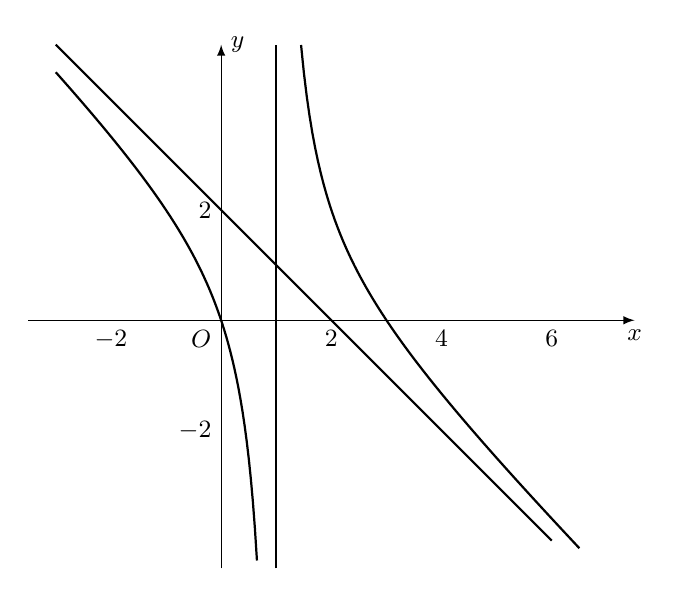
\begin{tikzpicture}[>=latex, scale=0.7]
    % 1. Hệ trục tọa độ
    \draw[->] (-3.5,0) -- (7.5,0) node[below] {\small $x$};
    \draw[->] (0,-4.5) -- (0,5) node[right] {\small $y$};
    \node[below left] at (0,0) {\small $O$};
    
    % 2. Vẽ đồ thị hàm số
    \draw[thick, samples=100, domain=-3:0.65] 
        plot (\x, {-\x+2 + 2/(\x -1)});
    \draw[thick, samples=100, domain=1.45:6.5] 
        plot (\x, {-\x+2 + 2/(\x -1)});
    \draw[thick, samples=100, domain=-3:6] 
        plot (\x, {-\x+2 });
    % 3. Đường tiệm cận
    \draw[thick] (1,-4.5) -- (1,5) ;
   
    
    % 4. Đánh dấu các điểm
    \node[left] at (0,-2) {\small $-2$};
     \node[left] at (0,2) {\small $2$};
    \node[below] at (-2,0) {\small $-2$};
    \node[below] at (2,0) {\small $2$};
    \node[below] at (4,0) {\small $4$};
    \node[below] at (6,0) {\small $6$};
\end{tikzpicture}
\end{center}

Đồ thị hàm số đã cho có bao nhiêu đường tiệm cận, phương trình cuaur các đường tiệm cận đó?}

\questionLinesManual{14}{4}{Cho hàm số \( y = f(x) \) có đồ thị hàm số như hình sau:

\begin{center}

\begin{tikzpicture}[>=latex, scale=0.8]
    % 1. Hệ trục tọa độ
    \draw[->] (-3.5,0) -- (5,0) node[below] {\small $x$};
    \draw[->] (0,-3.5) -- (0,5.5) node[right] {\small $y$};
    \node[below right] at (0,0) {\small $O$};
    
    % 2. Vẽ đồ thị hàm số (có tiệm cận xiên y = x - 1)
    \draw[thick, samples=100, domain=-3.2:0.76] 
        plot (\x, {\x  + 1/(\x-1)});
    \draw[thick, samples=100, domain=1.24:4.8] 
        plot (\x, {\x  + 1/(\x-1)});
    \draw[thick, samples=100, domain=-3.5:5] 
        plot (\x, {\x  });
    % 4. Đường tiệm cận đứng
    \draw[thick] (1,-3.5) -- (1,5.5);
    \draw[dashed] (0,1)--(1,1);
    % 5. Đánh dấu các điểm
   
    \node[below right] at (1,0) {\small $1$};
    \node[left] at (0,1) {\small $1$};
    \filldraw (1,0) circle (1.5pt);
    \filldraw (0,1) circle (1.5pt);
\end{tikzpicture}
\end{center}

Đường tiệm cận xiên của đồ thị hàm số là}

\questionLinesManual{10}{5}{Cho hàm số \( y = \dfrac{ax + b}{cx + d} \) (\( c \neq 0; ad - bc \neq 0 \)) có đồ thị như hình vẽ bên dưới.

\begin{center}
\begin{tikzpicture}[>=latex, scale=1]
    % 1. Hệ trục tọa độ
    \draw[->] (-3.5,0) -- (5.5,0) node[below] {\small $x$};
    \draw[->] (0,-3.5) -- (0,2.5) node[right] {\small $y$};
    \node[below left] at (0,0) {\small $O$};
    
    % 2. Vẽ đồ thị hàm số
    \draw[thick, samples=100, domain=-3.5:0.6] 
        plot (\x, {(-\x+2)/(\x - 1)});
    \draw[thick, samples=100, domain=1.3:5.5] 
        plot (\x, {(-\x+2)/(\x - 1)});
    
    % 3. Đường tiệm cận
    \draw[thick] (1,-3.5) -- (1,2.5);
    \draw[thick] (-3.5,-1) -- (5.5,-1);
    
    % 4. Đánh dấu các điểm
    \node[ below left] at (0,-1) {\small $-1$};
    \node[below left] at (1,0) {\small $1$};
     \node[below] at (2,0) {\small $2$};
      \node[below] at (0,-2) {\small $-2$};
    \filldraw (1,0) circle (1.5pt);
    \filldraw (2,0) circle (1.5pt);
    \filldraw (0,-1) circle (1.5pt);
    \filldraw (0,-2) circle (1.5pt);
\end{tikzpicture}
\end{center}

Đồ thị hàm số có đường tiệm cận ngang là:}{
    \begin{tasks}(4)
        \task \( y = 0 \)
        \task \( y = -1 \)
        \task \( x = -1 \)
        \task \( y = 1 \)
    \end{tasks}
}

% --- CÂU 52 ---
\questionLinesManual{10}{6}{Cho hàm số \( y = \dfrac{ax^2 + bx + c}{mx + n} \) có đồ thị như hình bên.

\begin{center}
\begin{tikzpicture}[>=latex, scale=1]
    % 1. Hệ trục tọa độ
    \draw[->] (-4.5,0) -- (4.5,0) node[below] {\small $x$};
    \draw[->] (0,-4.5) -- (0,4.5) node[right] {\small $y$};
    \node[below left] at (0,0) {\small $O$};
    
    % 2. Vẽ đồ thị hàm số
    \draw[thick, samples=100, domain=-4:-1.25] 
        plot (\x, {-\x - 1 + -1/(\x + 1)});
     \draw[thick, samples=100, domain=-0.75:3] 
        plot (\x, {-\x - 1 + -1/(\x + 1)});
     \draw[thick, samples=100, domain=-4:3] 
        plot (\x, {-\x - 1});
    \draw[thick] (-1,-4.5) -- (-1,4.5) ;
    
    % 5. Đánh dấu các điểm
    \node[below left] at (-1,0) {\small $-1$};
    \node[below] at (1,0) {\small $1$};
    \node[below left] at (0,-1) {\small $-1$};
    \filldraw (-1,0) circle (1.5pt);
    \filldraw (1,0) circle (1.5pt);
    \filldraw (0,-1) circle (1.5pt);
\end{tikzpicture}
\end{center}

Tiệm cận xiên của đồ thị hàm số đã cho là}{
    \begin{tasks}(4)
        \task \( y = -x + 1 \)
        \task \( y = x - 1 \)
        \task \( y = -x - 1 \)
        \task \( y = x + 1 \)
    \end{tasks}
}

\newpage
\drawdashlines{25}
\newpage

\questionLinesManual{5}{7}{Tiệm cận của đồ thị hàm số \( y = \dfrac{2x - 3}{x + 1} \) là đường thẳng có phương trình}
 
\questionLinesManual{5}{8}{Tiệm cận của đồ thị hàm số \( y = \dfrac{x - 1}{x - 3} \) là}

\questionLinesManual{7}{9}{Đường tiệm cận ngang của đồ thị hàm số \( y = 1 + \dfrac{2x + 1}{x + 2} \) có phương trình là:}

\questionLinesManual{8}{10}{Cho đồ thị hàm số \( y = \dfrac{2x^2 + x - 5}{x + 3} \) có đường tiệm cận xiên là đường thẳng \( \Delta : y = ax + b \) với \( a, b \in \mathbb{R}, a \neq 0 \). Giá trị của tổng \( a + b \) bằng}

\questionLinesManual{8}{11}{Đường tiệm cận xiên của đồ thị hàm số \( y = \dfrac{x^2 + 2x - 3}{x - 2} \) là}

\questionLinesManual{9}{12}{Đường tiệm cận xiên của đồ thị hàm số \( y = 2x - 1 + \dfrac{1}{x} \) có phương trình là:}

\questionLinesManual{8}{13}{Đồ thị hàm số \( y = 2x + 1 - \dfrac{3}{x + 1} \) có đường tiệm cận xiên là:}

\questionLinesManual{8}{14}{Cho hàm số \( y = 2x - 1 - \dfrac{3}{x + 2} \). Đường tiệm cận xiên của đồ thị hàm số đã cho là:}

\questionLinesManual{12}{15}{Cho hàm số \( y = \dfrac{ax + b}{cx + d} \), (\(ac \neq 0, ad - bc \neq 0\)) có bảng biến thiên như dưới đây.

\begin{center}
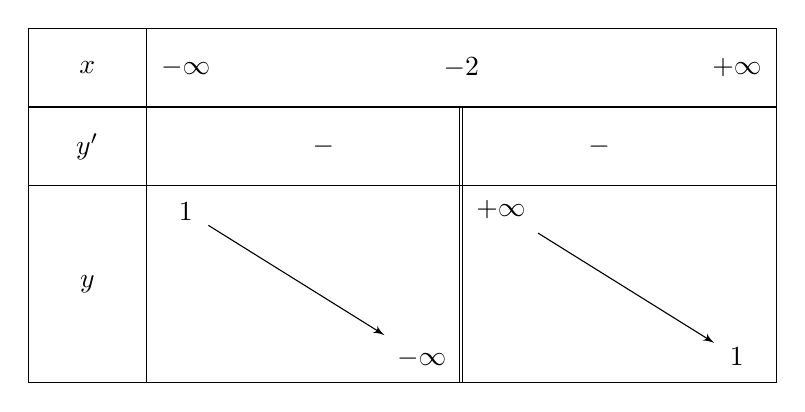
\begin{tikzpicture}
    \tkzTabInit[lgt=1.5, espcl=3.5]
    {$x$ /1, $y'$ /1, $y$ /2.5}
    {$-\infty$, $-2$, $+\infty$}
    \tkzTabLine{, -, d, -, }
    \tkzTabVar{+/ $1$ / , -D+/ $-\infty$ / $+\infty$ , -/ $1$ /}
\end{tikzpicture}
\end{center}

Đường tiệm cận đứng của đồ thị hàm số đã cho có phương trình là}

\questionLinesManual{8}{16}{Cho hàm số \( y = f(x) \) có bảng biến thiên như hình vẽ dưới đây.

\begin{center}
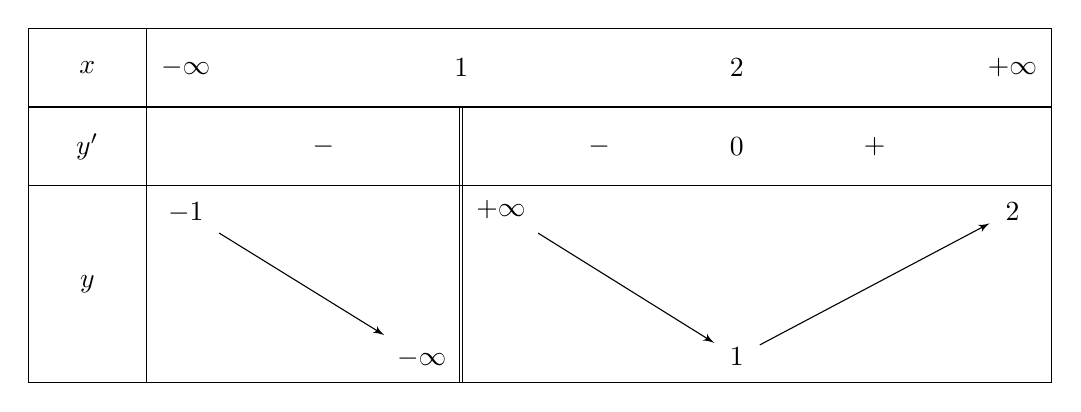
\begin{tikzpicture}
    \tkzTabInit[lgt=1.5, espcl=3.5]
    {$x$ /1, $y'$ /1, $y$ /2.5}
    {$-\infty$, $1$, $2$, $+\infty$}
    \tkzTabLine{, -, d, -, 0, +, }
    \tkzTabVar{+/ $-1$ / , -D+/ $-\infty$ / $+\infty$ , -/ $1$ / , +/ $2$ /}
\end{tikzpicture}
\end{center}

Đồ thị hàm số \( y = f(x) \) có bao nhiêu đường tiệm cận?}

\questionLinesManual{5}{17}{Cho hàm số \( f(x) \) xác định trên \( (-\infty; 0) \setminus \{-2\} \) và có bảng biến thiên bên dưới. Đồ thị hàm số đã cho có tổng số đường tiệm cận ngang và tiệm cận đứng là

\begin{center}
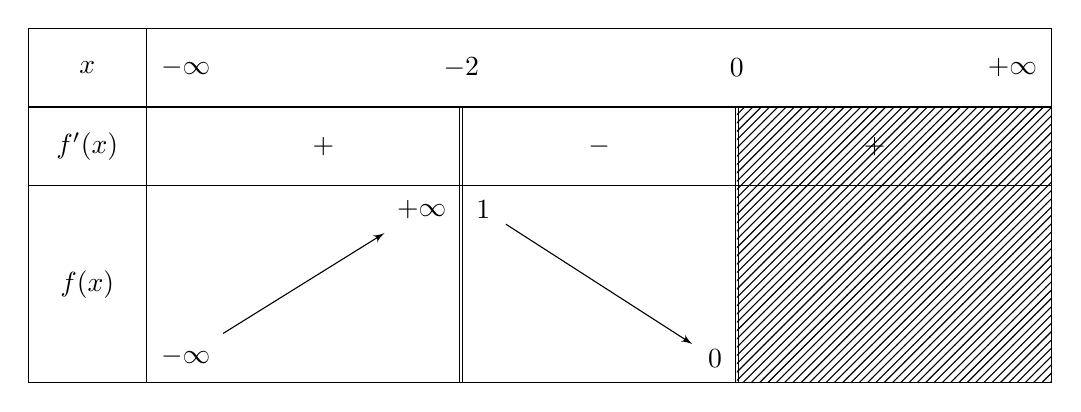
\begin{tikzpicture}
    \tkzTabInit[lgt=1.5, espcl=3.5]
    {$x$ /1, $f'(x)$ /1, $f(x)$ /2.5}
    {$-\infty$, $-2$, $0$, $+\infty$}
    \tkzTabLine{, +, d, -, d,+}
    \tkzTabVar{-/ $-\infty$ / , +D+/ $+\infty$ / $1$, -D/ $0$ /}
   \fill[pattern=north east lines](9,-4.5) rectangle (13,-1);
\end{tikzpicture}
\end{center}}

\questionLinesManual{8}{18}{Cho hàm số \( y = f(x) \) có bảng biến thiên như sau:

\begin{center}
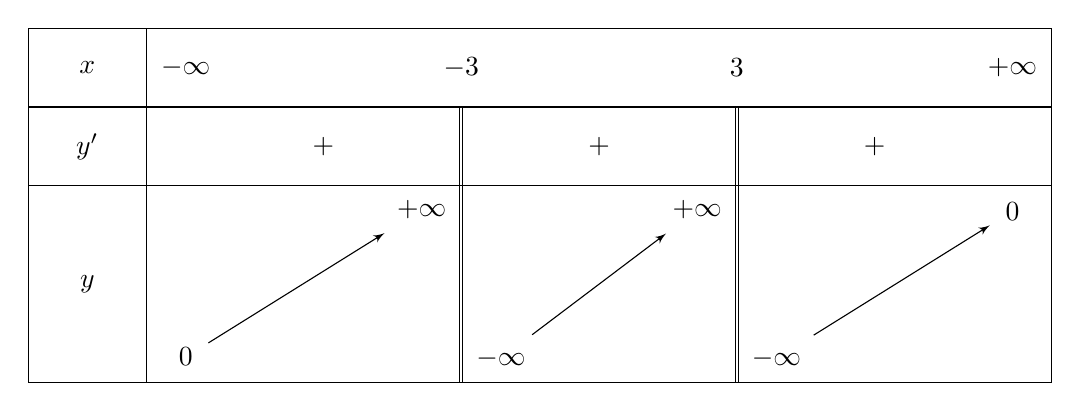
\begin{tikzpicture}
    \tkzTabInit[lgt=1.5, espcl=3.5]
    {$x$ /1, $y'$ /1, $y$ /2.5}
    {$-\infty$, $-3$, $3$, $+\infty$}
    \tkzTabLine{, +, d, +, d, +, }
    \tkzTabVar{-/ $0$ / , +D-/ $+\infty$ / $-\infty$, +D-/ $+\infty$ / $-\infty$, +/ $0$ /}
\end{tikzpicture}
\end{center}

Số đường tiệm cận đứng của đồ thị hàm số là}

\questionLinesManual{5}{19}{Cho hàm số \( y = f(x) \) có bảng biến thiên như sau

\begin{center}
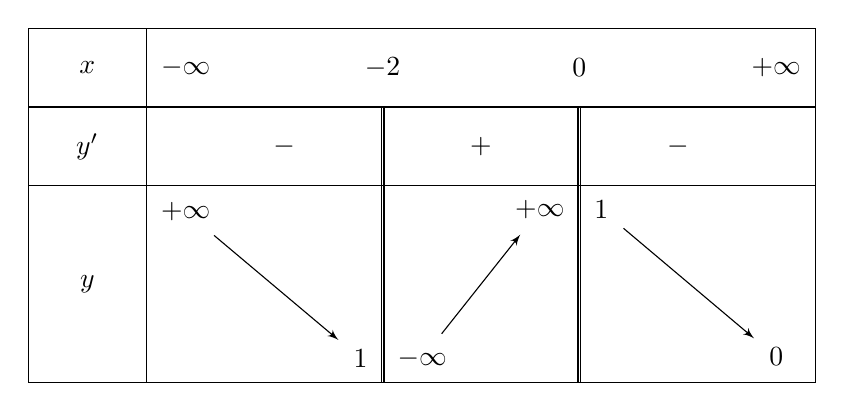
\begin{tikzpicture}
    \tkzTabInit[lgt=1.5, espcl=2.5]
    {$x$ /1, $y'$ /1, $y$ /2.5}
    {$-\infty$, $-2$, $0$, $+\infty$}
    \tkzTabLine{, -, d, +, d, -, }
    \tkzTabVar{+/ $+\infty$ / , -D-/ $1$ / $-\infty$/ ,+D+/ $+\infty$ / $1$ , -/ $0$ /}
\end{tikzpicture}
\end{center}

Tổng số đường tiệm cận đứng và tiệm cận ngang của đồ thị hàm số đã cho bằng}


\questionLinesManual{15}{20}{Cho hàm số có bảng biến thiên như hình sau

\begin{center}
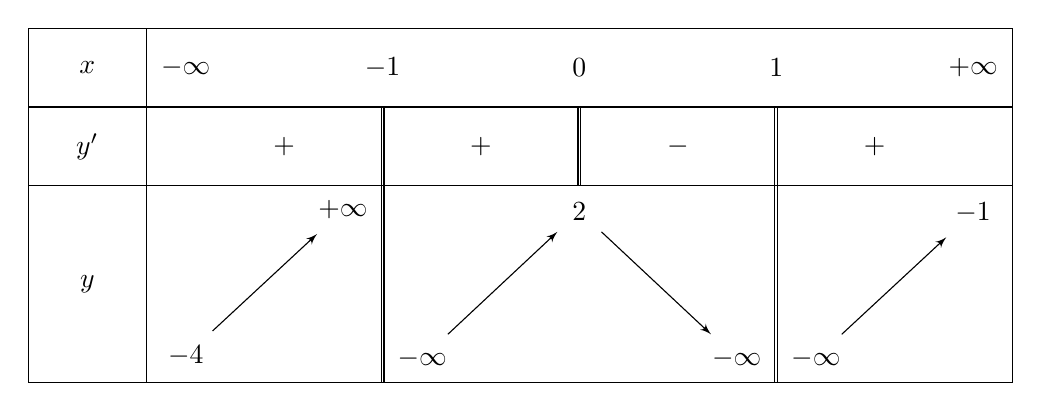
\begin{tikzpicture}
    \tkzTabInit[lgt=1.5, espcl=2.5]
    {$x$ /1, $y'$ /1, $y$ /2.5}
    {$-\infty$, $-1$, $0$, $1$, $+\infty$}
    \tkzTabLine{, +, d, +, d, -, d, +, }
    \tkzTabVar{-/ $-4$ / , +D-/ $+\infty$ /  $-\infty$,+ / $2$ ,  -D-/ $-\infty$ /$-\infty$ , +/ $-1$ /}
\end{tikzpicture}
\end{center}

Tổng số đường tiệm cận ngang và tiệm cận đứng của đồ thị hàm số \( y = f(x) \) là}

\newpage
\drawdashlines{25}
\end{document}